% Auto-generated by paper/05_run_statistical_tests.py

% Algorithm: NSGA-II (nsgaii)

% Source CSV: experiments/benchmark_paper.csv

%

% Include from main.tex with: % Auto-generated by paper/05_run_statistical_tests.py

% Algorithm: NSGA-II (nsgaii)

% Source CSV: experiments/benchmark_paper.csv

%

% Include from main.tex with: % Auto-generated by paper/05_run_statistical_tests.py

% Algorithm: NSGA-II (nsgaii)

% Source CSV: experiments/benchmark_paper.csv

%

% Include from main.tex with: % Auto-generated by paper/05_run_statistical_tests.py

% Algorithm: NSGA-II (nsgaii)

% Source CSV: experiments/benchmark_paper.csv

%

% Include from main.tex with: \input{stats_nsgaii.tex}



\begin{table}[htbp]
\centering
\caption{NSGA-II. Normalized hypervolume comparison with Wilcoxon signed-rank test results (Holm-corrected)}
\label{tab:stats_hypervolume_nsgaii}
\begin{tabular}{lccccc}
\toprule
\textbf{Problem} & \textbf{VAMOS} & \textbf{pymoo} & \textbf{p-value} & \textbf{$\hat{A}_{12}$} & \textbf{Significance} \\
\midrule
dtlz1 & 0.920 & \textbf{0.921} & 1.000 & 0.47 & \xmark \\
dtlz2 & 0.826 & \textbf{0.827} & 1.000 & 0.46 & \xmark \\
dtlz3 & \textbf{0.749} & 0.673 & 0.813 & 0.66 & \xmark \\
dtlz4 & 0.828 & \textbf{0.829} & 1.000 & 0.49 & \xmark \\
dtlz5 & 0.966 & \textbf{0.966} & 1.000 & 0.45 & \xmark \\
dtlz6 & 0.444 & \textbf{0.510} & 1.000 & 0.32 & \xmark \\
dtlz7 & \textbf{0.876} & 0.874 & 1.000 & 0.53 & \xmark \\
wfg1 & 0.353 & \textbf{0.430} & 1.000 & 0.36 & \xmark \\
wfg2 & 1.007 & \textbf{1.007} & 1.000 & 0.37 & \xmark \\
wfg3 & 0.971 & \textbf{0.973} & 1.000 & 0.35 & \xmark \\
wfg4 & 0.956 & \textbf{0.957} & 1.000 & 0.48 & \xmark \\
wfg5 & 0.826 & \textbf{0.826} & 0.513 & 0.32 & \xmark \\
wfg6 & 0.840 & \textbf{0.846} & 1.000 & 0.44 & \xmark \\
wfg7 & 0.963 & \textbf{0.964} & 1.000 & 0.41 & \xmark \\
wfg8 & \textbf{0.745} & 0.745 & 1.000 & 0.54 & \xmark \\
wfg9 & 0.714 & \textbf{0.714} & 1.000 & 0.48 & \xmark \\
zcat1 & 0.983 & \textbf{0.983} & 1.000 & 0.44 & \xmark \\
zcat10 & 0.951 & \textbf{0.951} & 1.000 & 0.43 & \xmark \\
zcat11 & 0.990 & \textbf{0.990} & 1.000 & 0.48 & \xmark \\
zcat12 & 0.989 & \textbf{0.990} & 1.000 & 0.45 & \xmark \\
zcat13 & 1.016 & \textbf{1.016} & 1.000 & 0.47 & \xmark \\
zcat14 & 0.977 & \textbf{0.977} & 1.000 & 0.36 & \xmark \\
zcat15 & 0.989 & \textbf{0.990} & 1.000 & 0.45 & \xmark \\
zcat16 & 0.987 & \textbf{0.988} & 1.000 & 0.40 & \xmark \\
zcat17 & 0.995 & \textbf{0.995} & 1.000 & 0.46 & \xmark \\
zcat18 & \textbf{0.990} & 0.990 & 1.000 & 0.52 & \xmark \\
zcat19 & 0.986 & \textbf{0.986} & 1.000 & 0.42 & \xmark \\
zcat2 & 0.992 & \textbf{0.992} & 1.000 & 0.49 & \xmark \\
zcat20 & \textbf{0.990} & 0.990 & 1.000 & 0.52 & \xmark \\
zcat3 & 0.983 & \textbf{0.983} & 1.000 & 0.37 & \xmark \\
zcat4 & 0.983 & \textbf{0.983} & 1.000 & 0.37 & \xmark \\
zcat5 & 0.995 & \textbf{0.995} & 1.000 & 0.46 & \xmark \\
zcat6 & 0.995 & \textbf{0.995} & 1.000 & 0.46 & \xmark \\
zcat7 & \textbf{0.990} & 0.990 & 1.000 & 0.52 & \xmark \\
zcat8 & 0.971 & \textbf{0.971} & 1.000 & 0.49 & \xmark \\
zcat9 & 0.971 & \textbf{0.971} & 1.000 & 0.49 & \xmark \\
zdt1 & 0.991 & \textbf{0.991} & 1.000 & 0.42 & \xmark \\
zdt2 & 0.982 & \textbf{0.982} & 1.000 & 0.44 & \xmark \\
zdt3 & 0.996 & \textbf{0.996} & 1.000 & 0.55 & \xmark \\
zdt4 & 1.001 & \textbf{1.001} & 1.000 & 0.43 & \xmark \\
zdt6 & 0.982 & \textbf{0.986} & $<$0.0001 & 0.00 & \cmark \\
\bottomrule
\end{tabular}
\end{table}

\begin{table}[htbp]
\centering
\caption{NSGA-II. IGD+ comparison with Wilcoxon signed-rank test results (Holm-corrected). Lower is better}
\label{tab:stats_igd_plus_nsgaii}
\begin{tabular}{lccccc}
\toprule
\textbf{Problem} & \textbf{VAMOS} & \textbf{pymoo} & \textbf{p-value} & \textbf{$\hat{A}_{12}$} & \textbf{Significance} \\
\midrule
dtlz1 & 0.0181 & \textbf{0.0179} & 1.000 & 0.53 &  \xmark \\
dtlz2 & 0.0357 & \textbf{0.0352} & 1.000 & 0.56 &  \xmark \\
dtlz3 & \textbf{0.0518} & 0.0716 & 0.834 & 0.32 &  \xmark \\
dtlz4 & 0.0357 & \textbf{0.0351} & 1.000 & 0.54 &  \xmark \\
dtlz5 & 0.0029 & \textbf{0.0029} & 1.000 & 0.51 &  \xmark \\
dtlz6 & 0.0996 & \textbf{0.0837} & 1.000 & 0.67 &  \xmark \\
dtlz7 & 0.0350 & \textbf{0.0350} & 1.000 & 0.56 &  \xmark \\
wfg1 & 0.7451 & \textbf{0.6949} & 1.000 & 0.65 &  \xmark \\
wfg2 & 0.2162 & \textbf{0.2155} & 1.000 & 0.64 &  \xmark \\
wfg3 & 0.0206 & \textbf{0.0191} & 1.000 & 0.65 &  \xmark \\
wfg4 & 0.0133 & \textbf{0.0128} & 1.000 & 0.53 &  \xmark \\
wfg5 & \textbf{0.0699} & 0.0700 & 1.000 & 0.51 &  \xmark \\
wfg6 & 0.0600 & \textbf{0.0573} & 1.000 & 0.59 &  \xmark \\
wfg7 & 0.0106 & \textbf{0.0103} & 1.000 & 0.58 &  \xmark \\
wfg8 & \textbf{0.1463} & 0.1485 & 1.000 & 0.45 &  \xmark \\
wfg9 & \textbf{0.1263} & 0.1264 & 1.000 & 0.51 &  \xmark \\
zcat1 & 0.0074 & \textbf{0.0073} & 1.000 & 0.58 &  \xmark \\
zcat10 & 0.0033 & \textbf{0.0032} & 1.000 & 0.57 &  \xmark \\
zcat11 & 0.0049 & \textbf{0.0049} & 1.000 & 0.49 &  \xmark \\
zcat12 & 0.0050 & \textbf{0.0049} & 1.000 & 0.52 &  \xmark \\
zcat13 & 0.0038 & \textbf{0.0037} & 1.000 & 0.57 &  \xmark \\
zcat14 & 0.0070 & \textbf{0.0069} & 1.000 & 0.64 &  \xmark \\
zcat15 & 0.0050 & \textbf{0.0050} & 1.000 & 0.52 &  \xmark \\
zcat16 & 0.0048 & \textbf{0.0046} & 1.000 & 0.58 &  \xmark \\
zcat17 & 0.0040 & \textbf{0.0040} & 1.000 & 0.51 &  \xmark \\
zcat18 & \textbf{0.0044} & 0.0044 & 1.000 & 0.51 &  \xmark \\
zcat19 & 0.0062 & \textbf{0.0061} & 1.000 & 0.58 &  \xmark \\
zcat2 & 0.0059 & \textbf{0.0059} & 1.000 & 0.52 &  \xmark \\
zcat20 & \textbf{0.0045} & 0.0045 & 1.000 & 0.52 &  \xmark \\
zcat3 & 0.0074 & \textbf{0.0072} & 1.000 & 0.63 &  \xmark \\
zcat4 & 0.0074 & \textbf{0.0072} & 1.000 & 0.63 &  \xmark \\
zcat5 & 0.0040 & \textbf{0.0040} & 1.000 & 0.53 &  \xmark \\
zcat6 & 0.0027 & \textbf{0.0026} & 1.000 & 0.63 &  \xmark \\
zcat7 & \textbf{0.0044} & 0.0044 & 1.000 & 0.52 &  \xmark \\
zcat8 & 0.0057 & \textbf{0.0056} & 1.000 & 0.51 &  \xmark \\
zcat9 & 0.0057 & \textbf{0.0057} & 1.000 & 0.50 &  \xmark \\
zdt1 & 0.0032 & \textbf{0.0031} & 1.000 & 0.53 &  \xmark \\
zdt2 & 0.0030 & \textbf{0.0030} & 1.000 & 0.53 &  \xmark \\
zdt3 & \textbf{0.0015} & 0.0015 & 1.000 & 0.45 &  \xmark \\
zdt4 & 0.0008 & \textbf{0.0008} & 1.000 & 0.59 &  \xmark \\
zdt6 & 0.0031 & \textbf{0.0024} & $<$0.0001 & 1.00 & \checkmark \\
\bottomrule
\end{tabular}
\end{table}

\begin{table}[htbp]
\centering
\caption{Normalized hypervolume equivalence summary (paired bootstrap 90\% CI; equivalence margin $\pm 1\%$ relative)}
\label{tab:hv_equivalence_summary_nsgaii}
\resizebox{\columnwidth}{!}{%
\begin{tabular}{lccc}
\toprule
\textbf{Framework} & \textbf{Eq.\ problems} & \textbf{Non-inf.\ problems} & \textbf{Median $\Delta$HV (\%)} \\
\midrule
\textit{pymoo} & 37/41 & 38/41 & -0.01 \\
\textit{jMetalPy} & 35/41 & 35/41 & -0.02 \\
\textit{DEAP} & 33/41 & 37/41 & -0.01 \\
\textit{Platypus} & 33/41 & 38/41 & +0.05 \\
\bottomrule
\end{tabular}%
}
\end{table}

\begin{table}[htbp]
\centering
\caption{Robustness summary for normalized hypervolume across seeds (median across problems). ``Near-best'' is defined per problem as HV $\ge 0.99 \cdot \max$ median(HV) among frameworks}
\label{tab:hv_robustness_summary_nsgaii}
\begin{tabular}{lcc}
\toprule
\textbf{Framework} & \textbf{Median IQR(HV)} & \textbf{Median \% seeds near-best} \\
\midrule
VAMOS & 0.001 & 100.0 \\
\textit{pymoo} & 0.001 & 100.0 \\
\textit{jMetalPy} & 0.002 & 100.0 \\
\textit{DEAP} & 0.001 & 100.0 \\
\textit{Platypus} & 0.001 & 100.0 \\
\bottomrule
\end{tabular}
\end{table}

\begin{figure}[htbp]
  \centering
  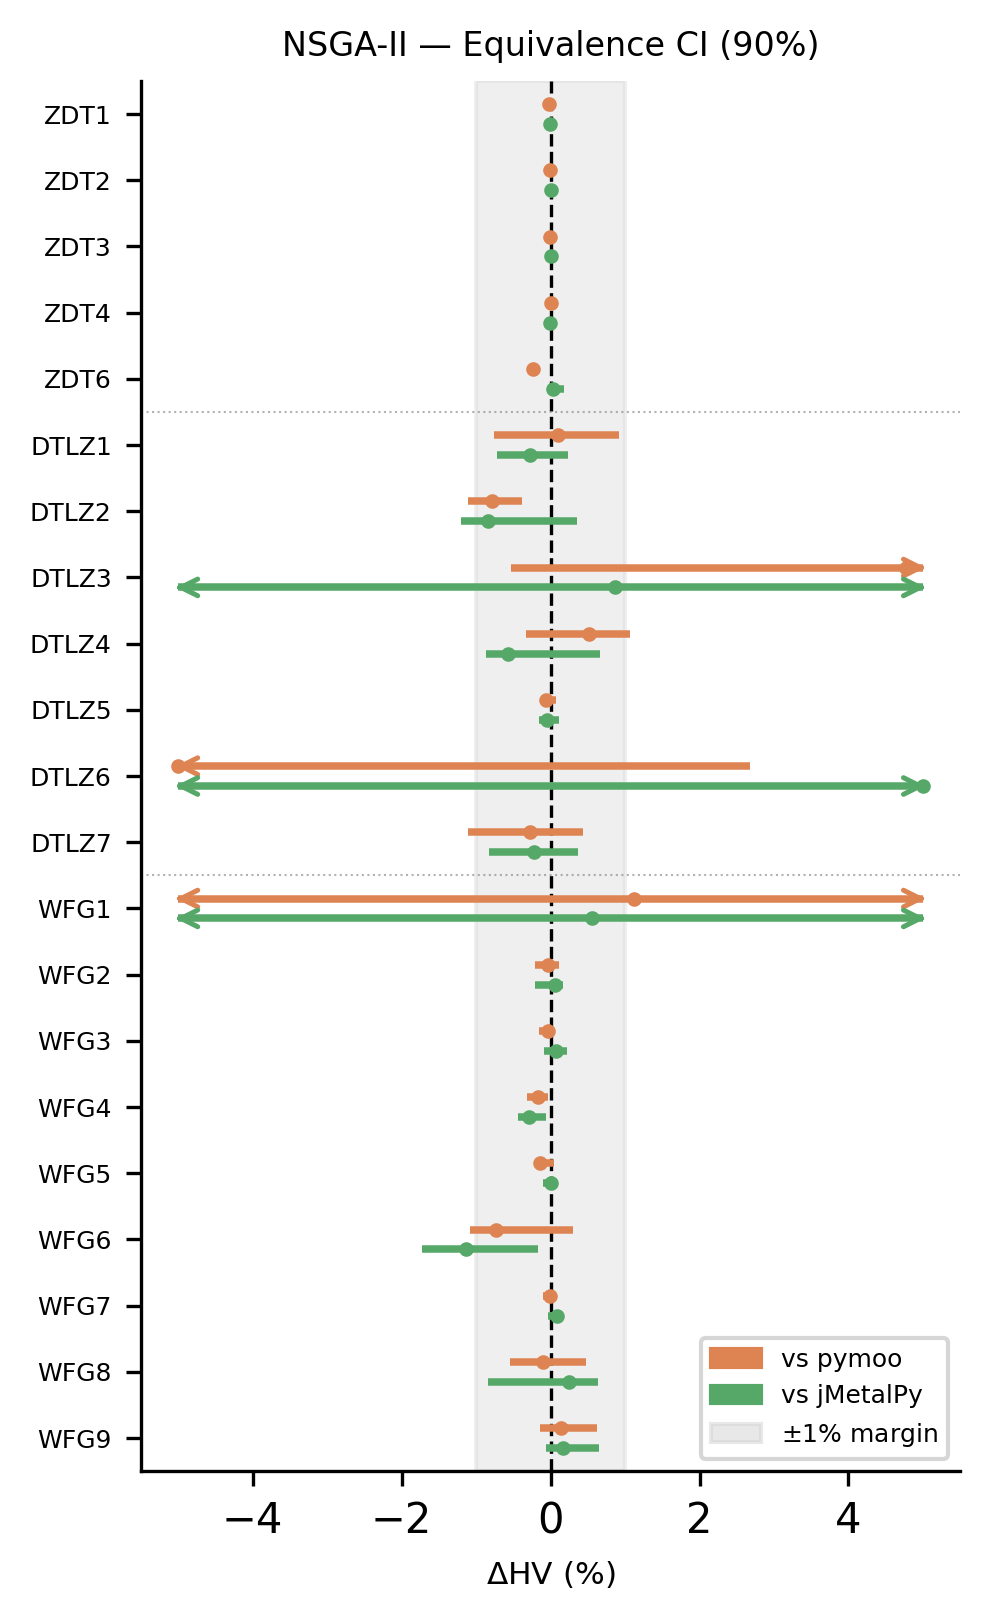
\includegraphics[width=\columnwidth]{figures/forest_ci_nsgaii.png}
  \caption{NSGA-II. Per-problem paired bootstrap 90\% confidence intervals for the relative normalized hypervolume difference $\Delta = (\HV_{\text{\VAMOS}} - \HV_{\text{fw}})/\HV_{\text{fw}}$, reported in percent. The shaded band marks the $\pm 1\%$ equivalence margin; intervals falling entirely within this band indicate statistical equivalence}
  \label{fig:forest_ci_nsgaii}
\end{figure}




\begin{table}[htbp]
\centering
\caption{NSGA-II. Normalized hypervolume comparison with Wilcoxon signed-rank test results (Holm-corrected)}
\label{tab:stats_hypervolume_nsgaii}
\begin{tabular}{lccccc}
\toprule
\textbf{Problem} & \textbf{VAMOS} & \textbf{pymoo} & \textbf{p-value} & \textbf{$\hat{A}_{12}$} & \textbf{Significance} \\
\midrule
dtlz1 & 0.920 & \textbf{0.921} & 1.000 & 0.47 & \xmark \\
dtlz2 & 0.826 & \textbf{0.827} & 1.000 & 0.46 & \xmark \\
dtlz3 & \textbf{0.749} & 0.673 & 0.813 & 0.66 & \xmark \\
dtlz4 & 0.828 & \textbf{0.829} & 1.000 & 0.49 & \xmark \\
dtlz5 & 0.966 & \textbf{0.966} & 1.000 & 0.45 & \xmark \\
dtlz6 & 0.444 & \textbf{0.510} & 1.000 & 0.32 & \xmark \\
dtlz7 & \textbf{0.876} & 0.874 & 1.000 & 0.53 & \xmark \\
wfg1 & 0.353 & \textbf{0.430} & 1.000 & 0.36 & \xmark \\
wfg2 & 1.007 & \textbf{1.007} & 1.000 & 0.37 & \xmark \\
wfg3 & 0.971 & \textbf{0.973} & 1.000 & 0.35 & \xmark \\
wfg4 & 0.956 & \textbf{0.957} & 1.000 & 0.48 & \xmark \\
wfg5 & 0.826 & \textbf{0.826} & 0.513 & 0.32 & \xmark \\
wfg6 & 0.840 & \textbf{0.846} & 1.000 & 0.44 & \xmark \\
wfg7 & 0.963 & \textbf{0.964} & 1.000 & 0.41 & \xmark \\
wfg8 & \textbf{0.745} & 0.745 & 1.000 & 0.54 & \xmark \\
wfg9 & 0.714 & \textbf{0.714} & 1.000 & 0.48 & \xmark \\
zcat1 & 0.983 & \textbf{0.983} & 1.000 & 0.44 & \xmark \\
zcat10 & 0.951 & \textbf{0.951} & 1.000 & 0.43 & \xmark \\
zcat11 & 0.990 & \textbf{0.990} & 1.000 & 0.48 & \xmark \\
zcat12 & 0.989 & \textbf{0.990} & 1.000 & 0.45 & \xmark \\
zcat13 & 1.016 & \textbf{1.016} & 1.000 & 0.47 & \xmark \\
zcat14 & 0.977 & \textbf{0.977} & 1.000 & 0.36 & \xmark \\
zcat15 & 0.989 & \textbf{0.990} & 1.000 & 0.45 & \xmark \\
zcat16 & 0.987 & \textbf{0.988} & 1.000 & 0.40 & \xmark \\
zcat17 & 0.995 & \textbf{0.995} & 1.000 & 0.46 & \xmark \\
zcat18 & \textbf{0.990} & 0.990 & 1.000 & 0.52 & \xmark \\
zcat19 & 0.986 & \textbf{0.986} & 1.000 & 0.42 & \xmark \\
zcat2 & 0.992 & \textbf{0.992} & 1.000 & 0.49 & \xmark \\
zcat20 & \textbf{0.990} & 0.990 & 1.000 & 0.52 & \xmark \\
zcat3 & 0.983 & \textbf{0.983} & 1.000 & 0.37 & \xmark \\
zcat4 & 0.983 & \textbf{0.983} & 1.000 & 0.37 & \xmark \\
zcat5 & 0.995 & \textbf{0.995} & 1.000 & 0.46 & \xmark \\
zcat6 & 0.995 & \textbf{0.995} & 1.000 & 0.46 & \xmark \\
zcat7 & \textbf{0.990} & 0.990 & 1.000 & 0.52 & \xmark \\
zcat8 & 0.971 & \textbf{0.971} & 1.000 & 0.49 & \xmark \\
zcat9 & 0.971 & \textbf{0.971} & 1.000 & 0.49 & \xmark \\
zdt1 & 0.991 & \textbf{0.991} & 1.000 & 0.42 & \xmark \\
zdt2 & 0.982 & \textbf{0.982} & 1.000 & 0.44 & \xmark \\
zdt3 & 0.996 & \textbf{0.996} & 1.000 & 0.55 & \xmark \\
zdt4 & 1.001 & \textbf{1.001} & 1.000 & 0.43 & \xmark \\
zdt6 & 0.982 & \textbf{0.986} & $<$0.0001 & 0.00 & \cmark \\
\bottomrule
\end{tabular}
\end{table}

\begin{table}[htbp]
\centering
\caption{NSGA-II. IGD+ comparison with Wilcoxon signed-rank test results (Holm-corrected). Lower is better}
\label{tab:stats_igd_plus_nsgaii}
\begin{tabular}{lccccc}
\toprule
\textbf{Problem} & \textbf{VAMOS} & \textbf{pymoo} & \textbf{p-value} & \textbf{$\hat{A}_{12}$} & \textbf{Significance} \\
\midrule
dtlz1 & 0.0181 & \textbf{0.0179} & 1.000 & 0.53 &  \xmark \\
dtlz2 & 0.0357 & \textbf{0.0352} & 1.000 & 0.56 &  \xmark \\
dtlz3 & \textbf{0.0518} & 0.0716 & 0.834 & 0.32 &  \xmark \\
dtlz4 & 0.0357 & \textbf{0.0351} & 1.000 & 0.54 &  \xmark \\
dtlz5 & 0.0029 & \textbf{0.0029} & 1.000 & 0.51 &  \xmark \\
dtlz6 & 0.0996 & \textbf{0.0837} & 1.000 & 0.67 &  \xmark \\
dtlz7 & 0.0350 & \textbf{0.0350} & 1.000 & 0.56 &  \xmark \\
wfg1 & 0.7451 & \textbf{0.6949} & 1.000 & 0.65 &  \xmark \\
wfg2 & 0.2162 & \textbf{0.2155} & 1.000 & 0.64 &  \xmark \\
wfg3 & 0.0206 & \textbf{0.0191} & 1.000 & 0.65 &  \xmark \\
wfg4 & 0.0133 & \textbf{0.0128} & 1.000 & 0.53 &  \xmark \\
wfg5 & \textbf{0.0699} & 0.0700 & 1.000 & 0.51 &  \xmark \\
wfg6 & 0.0600 & \textbf{0.0573} & 1.000 & 0.59 &  \xmark \\
wfg7 & 0.0106 & \textbf{0.0103} & 1.000 & 0.58 &  \xmark \\
wfg8 & \textbf{0.1463} & 0.1485 & 1.000 & 0.45 &  \xmark \\
wfg9 & \textbf{0.1263} & 0.1264 & 1.000 & 0.51 &  \xmark \\
zcat1 & 0.0074 & \textbf{0.0073} & 1.000 & 0.58 &  \xmark \\
zcat10 & 0.0033 & \textbf{0.0032} & 1.000 & 0.57 &  \xmark \\
zcat11 & 0.0049 & \textbf{0.0049} & 1.000 & 0.49 &  \xmark \\
zcat12 & 0.0050 & \textbf{0.0049} & 1.000 & 0.52 &  \xmark \\
zcat13 & 0.0038 & \textbf{0.0037} & 1.000 & 0.57 &  \xmark \\
zcat14 & 0.0070 & \textbf{0.0069} & 1.000 & 0.64 &  \xmark \\
zcat15 & 0.0050 & \textbf{0.0050} & 1.000 & 0.52 &  \xmark \\
zcat16 & 0.0048 & \textbf{0.0046} & 1.000 & 0.58 &  \xmark \\
zcat17 & 0.0040 & \textbf{0.0040} & 1.000 & 0.51 &  \xmark \\
zcat18 & \textbf{0.0044} & 0.0044 & 1.000 & 0.51 &  \xmark \\
zcat19 & 0.0062 & \textbf{0.0061} & 1.000 & 0.58 &  \xmark \\
zcat2 & 0.0059 & \textbf{0.0059} & 1.000 & 0.52 &  \xmark \\
zcat20 & \textbf{0.0045} & 0.0045 & 1.000 & 0.52 &  \xmark \\
zcat3 & 0.0074 & \textbf{0.0072} & 1.000 & 0.63 &  \xmark \\
zcat4 & 0.0074 & \textbf{0.0072} & 1.000 & 0.63 &  \xmark \\
zcat5 & 0.0040 & \textbf{0.0040} & 1.000 & 0.53 &  \xmark \\
zcat6 & 0.0027 & \textbf{0.0026} & 1.000 & 0.63 &  \xmark \\
zcat7 & \textbf{0.0044} & 0.0044 & 1.000 & 0.52 &  \xmark \\
zcat8 & 0.0057 & \textbf{0.0056} & 1.000 & 0.51 &  \xmark \\
zcat9 & 0.0057 & \textbf{0.0057} & 1.000 & 0.50 &  \xmark \\
zdt1 & 0.0032 & \textbf{0.0031} & 1.000 & 0.53 &  \xmark \\
zdt2 & 0.0030 & \textbf{0.0030} & 1.000 & 0.53 &  \xmark \\
zdt3 & \textbf{0.0015} & 0.0015 & 1.000 & 0.45 &  \xmark \\
zdt4 & 0.0008 & \textbf{0.0008} & 1.000 & 0.59 &  \xmark \\
zdt6 & 0.0031 & \textbf{0.0024} & $<$0.0001 & 1.00 & \checkmark \\
\bottomrule
\end{tabular}
\end{table}

\begin{table}[htbp]
\centering
\caption{Normalized hypervolume equivalence summary (paired bootstrap 90\% CI; equivalence margin $\pm 1\%$ relative)}
\label{tab:hv_equivalence_summary_nsgaii}
\resizebox{\columnwidth}{!}{%
\begin{tabular}{lccc}
\toprule
\textbf{Framework} & \textbf{Eq.\ problems} & \textbf{Non-inf.\ problems} & \textbf{Median $\Delta$HV (\%)} \\
\midrule
\textit{pymoo} & 37/41 & 38/41 & -0.01 \\
\textit{jMetalPy} & 35/41 & 35/41 & -0.02 \\
\textit{DEAP} & 33/41 & 37/41 & -0.01 \\
\textit{Platypus} & 33/41 & 38/41 & +0.05 \\
\bottomrule
\end{tabular}%
}
\end{table}

\begin{table}[htbp]
\centering
\caption{Robustness summary for normalized hypervolume across seeds (median across problems). ``Near-best'' is defined per problem as HV $\ge 0.99 \cdot \max$ median(HV) among frameworks}
\label{tab:hv_robustness_summary_nsgaii}
\begin{tabular}{lcc}
\toprule
\textbf{Framework} & \textbf{Median IQR(HV)} & \textbf{Median \% seeds near-best} \\
\midrule
VAMOS & 0.001 & 100.0 \\
\textit{pymoo} & 0.001 & 100.0 \\
\textit{jMetalPy} & 0.002 & 100.0 \\
\textit{DEAP} & 0.001 & 100.0 \\
\textit{Platypus} & 0.001 & 100.0 \\
\bottomrule
\end{tabular}
\end{table}

\begin{figure}[htbp]
  \centering
  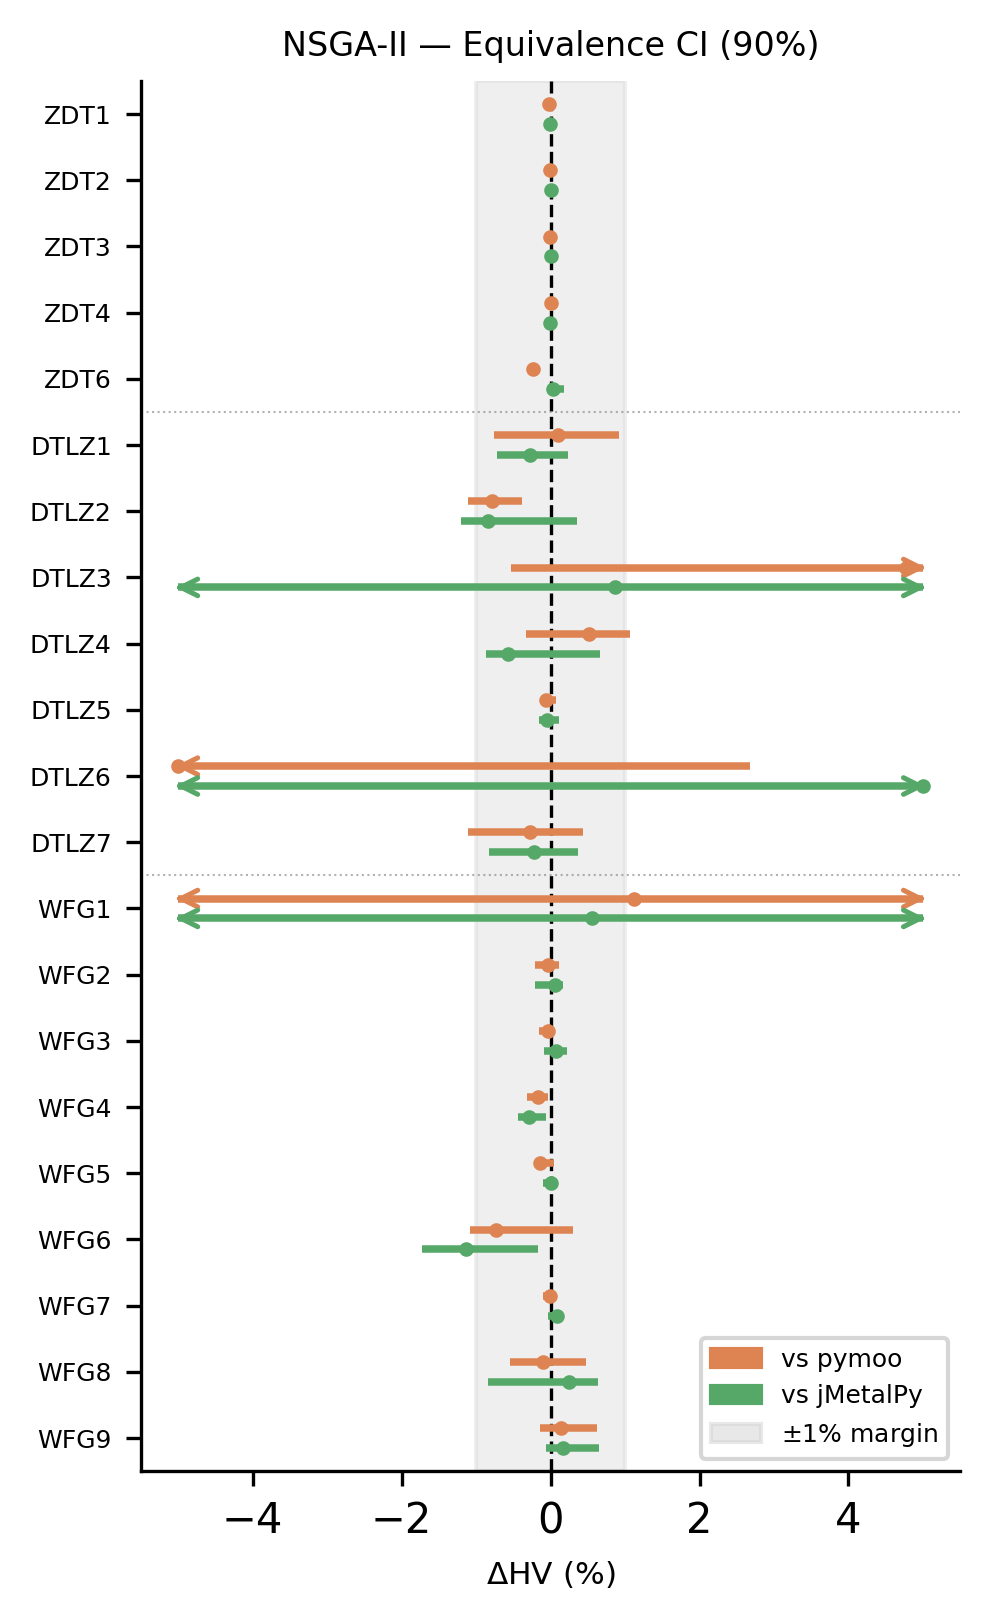
\includegraphics[width=\columnwidth]{figures/forest_ci_nsgaii.png}
  \caption{NSGA-II. Per-problem paired bootstrap 90\% confidence intervals for the relative normalized hypervolume difference $\Delta = (\HV_{\text{\VAMOS}} - \HV_{\text{fw}})/\HV_{\text{fw}}$, reported in percent. The shaded band marks the $\pm 1\%$ equivalence margin; intervals falling entirely within this band indicate statistical equivalence}
  \label{fig:forest_ci_nsgaii}
\end{figure}




\begin{table}[htbp]
\centering
\caption{NSGA-II. Normalized hypervolume comparison with Wilcoxon signed-rank test results (Holm-corrected)}
\label{tab:stats_hypervolume_nsgaii}
\begin{tabular}{lccccc}
\toprule
\textbf{Problem} & \textbf{VAMOS} & \textbf{pymoo} & \textbf{p-value} & \textbf{$\hat{A}_{12}$} & \textbf{Significance} \\
\midrule
dtlz1 & 0.920 & \textbf{0.921} & 1.000 & 0.47 & \xmark \\
dtlz2 & 0.826 & \textbf{0.827} & 1.000 & 0.46 & \xmark \\
dtlz3 & \textbf{0.749} & 0.673 & 0.813 & 0.66 & \xmark \\
dtlz4 & 0.828 & \textbf{0.829} & 1.000 & 0.49 & \xmark \\
dtlz5 & 0.966 & \textbf{0.966} & 1.000 & 0.45 & \xmark \\
dtlz6 & 0.444 & \textbf{0.510} & 1.000 & 0.32 & \xmark \\
dtlz7 & \textbf{0.876} & 0.874 & 1.000 & 0.53 & \xmark \\
wfg1 & 0.353 & \textbf{0.430} & 1.000 & 0.36 & \xmark \\
wfg2 & 1.007 & \textbf{1.007} & 1.000 & 0.37 & \xmark \\
wfg3 & 0.971 & \textbf{0.973} & 1.000 & 0.35 & \xmark \\
wfg4 & 0.956 & \textbf{0.957} & 1.000 & 0.48 & \xmark \\
wfg5 & 0.826 & \textbf{0.826} & 0.513 & 0.32 & \xmark \\
wfg6 & 0.840 & \textbf{0.846} & 1.000 & 0.44 & \xmark \\
wfg7 & 0.963 & \textbf{0.964} & 1.000 & 0.41 & \xmark \\
wfg8 & \textbf{0.745} & 0.745 & 1.000 & 0.54 & \xmark \\
wfg9 & 0.714 & \textbf{0.714} & 1.000 & 0.48 & \xmark \\
zcat1 & 0.983 & \textbf{0.983} & 1.000 & 0.44 & \xmark \\
zcat10 & 0.951 & \textbf{0.951} & 1.000 & 0.43 & \xmark \\
zcat11 & 0.990 & \textbf{0.990} & 1.000 & 0.48 & \xmark \\
zcat12 & 0.989 & \textbf{0.990} & 1.000 & 0.45 & \xmark \\
zcat13 & 1.016 & \textbf{1.016} & 1.000 & 0.47 & \xmark \\
zcat14 & 0.977 & \textbf{0.977} & 1.000 & 0.36 & \xmark \\
zcat15 & 0.989 & \textbf{0.990} & 1.000 & 0.45 & \xmark \\
zcat16 & 0.987 & \textbf{0.988} & 1.000 & 0.40 & \xmark \\
zcat17 & 0.995 & \textbf{0.995} & 1.000 & 0.46 & \xmark \\
zcat18 & \textbf{0.990} & 0.990 & 1.000 & 0.52 & \xmark \\
zcat19 & 0.986 & \textbf{0.986} & 1.000 & 0.42 & \xmark \\
zcat2 & 0.992 & \textbf{0.992} & 1.000 & 0.49 & \xmark \\
zcat20 & \textbf{0.990} & 0.990 & 1.000 & 0.52 & \xmark \\
zcat3 & 0.983 & \textbf{0.983} & 1.000 & 0.37 & \xmark \\
zcat4 & 0.983 & \textbf{0.983} & 1.000 & 0.37 & \xmark \\
zcat5 & 0.995 & \textbf{0.995} & 1.000 & 0.46 & \xmark \\
zcat6 & 0.995 & \textbf{0.995} & 1.000 & 0.46 & \xmark \\
zcat7 & \textbf{0.990} & 0.990 & 1.000 & 0.52 & \xmark \\
zcat8 & 0.971 & \textbf{0.971} & 1.000 & 0.49 & \xmark \\
zcat9 & 0.971 & \textbf{0.971} & 1.000 & 0.49 & \xmark \\
zdt1 & 0.991 & \textbf{0.991} & 1.000 & 0.42 & \xmark \\
zdt2 & 0.982 & \textbf{0.982} & 1.000 & 0.44 & \xmark \\
zdt3 & 0.996 & \textbf{0.996} & 1.000 & 0.55 & \xmark \\
zdt4 & 1.001 & \textbf{1.001} & 1.000 & 0.43 & \xmark \\
zdt6 & 0.982 & \textbf{0.986} & $<$0.0001 & 0.00 & \cmark \\
\bottomrule
\end{tabular}
\end{table}

\begin{table}[htbp]
\centering
\caption{NSGA-II. IGD+ comparison with Wilcoxon signed-rank test results (Holm-corrected). Lower is better}
\label{tab:stats_igd_plus_nsgaii}
\begin{tabular}{lccccc}
\toprule
\textbf{Problem} & \textbf{VAMOS} & \textbf{pymoo} & \textbf{p-value} & \textbf{$\hat{A}_{12}$} & \textbf{Significance} \\
\midrule
dtlz1 & 0.0181 & \textbf{0.0179} & 1.000 & 0.53 &  \xmark \\
dtlz2 & 0.0357 & \textbf{0.0352} & 1.000 & 0.56 &  \xmark \\
dtlz3 & \textbf{0.0518} & 0.0716 & 0.834 & 0.32 &  \xmark \\
dtlz4 & 0.0357 & \textbf{0.0351} & 1.000 & 0.54 &  \xmark \\
dtlz5 & 0.0029 & \textbf{0.0029} & 1.000 & 0.51 &  \xmark \\
dtlz6 & 0.0996 & \textbf{0.0837} & 1.000 & 0.67 &  \xmark \\
dtlz7 & 0.0350 & \textbf{0.0350} & 1.000 & 0.56 &  \xmark \\
wfg1 & 0.7451 & \textbf{0.6949} & 1.000 & 0.65 &  \xmark \\
wfg2 & 0.2162 & \textbf{0.2155} & 1.000 & 0.64 &  \xmark \\
wfg3 & 0.0206 & \textbf{0.0191} & 1.000 & 0.65 &  \xmark \\
wfg4 & 0.0133 & \textbf{0.0128} & 1.000 & 0.53 &  \xmark \\
wfg5 & \textbf{0.0699} & 0.0700 & 1.000 & 0.51 &  \xmark \\
wfg6 & 0.0600 & \textbf{0.0573} & 1.000 & 0.59 &  \xmark \\
wfg7 & 0.0106 & \textbf{0.0103} & 1.000 & 0.58 &  \xmark \\
wfg8 & \textbf{0.1463} & 0.1485 & 1.000 & 0.45 &  \xmark \\
wfg9 & \textbf{0.1263} & 0.1264 & 1.000 & 0.51 &  \xmark \\
zcat1 & 0.0074 & \textbf{0.0073} & 1.000 & 0.58 &  \xmark \\
zcat10 & 0.0033 & \textbf{0.0032} & 1.000 & 0.57 &  \xmark \\
zcat11 & 0.0049 & \textbf{0.0049} & 1.000 & 0.49 &  \xmark \\
zcat12 & 0.0050 & \textbf{0.0049} & 1.000 & 0.52 &  \xmark \\
zcat13 & 0.0038 & \textbf{0.0037} & 1.000 & 0.57 &  \xmark \\
zcat14 & 0.0070 & \textbf{0.0069} & 1.000 & 0.64 &  \xmark \\
zcat15 & 0.0050 & \textbf{0.0050} & 1.000 & 0.52 &  \xmark \\
zcat16 & 0.0048 & \textbf{0.0046} & 1.000 & 0.58 &  \xmark \\
zcat17 & 0.0040 & \textbf{0.0040} & 1.000 & 0.51 &  \xmark \\
zcat18 & \textbf{0.0044} & 0.0044 & 1.000 & 0.51 &  \xmark \\
zcat19 & 0.0062 & \textbf{0.0061} & 1.000 & 0.58 &  \xmark \\
zcat2 & 0.0059 & \textbf{0.0059} & 1.000 & 0.52 &  \xmark \\
zcat20 & \textbf{0.0045} & 0.0045 & 1.000 & 0.52 &  \xmark \\
zcat3 & 0.0074 & \textbf{0.0072} & 1.000 & 0.63 &  \xmark \\
zcat4 & 0.0074 & \textbf{0.0072} & 1.000 & 0.63 &  \xmark \\
zcat5 & 0.0040 & \textbf{0.0040} & 1.000 & 0.53 &  \xmark \\
zcat6 & 0.0027 & \textbf{0.0026} & 1.000 & 0.63 &  \xmark \\
zcat7 & \textbf{0.0044} & 0.0044 & 1.000 & 0.52 &  \xmark \\
zcat8 & 0.0057 & \textbf{0.0056} & 1.000 & 0.51 &  \xmark \\
zcat9 & 0.0057 & \textbf{0.0057} & 1.000 & 0.50 &  \xmark \\
zdt1 & 0.0032 & \textbf{0.0031} & 1.000 & 0.53 &  \xmark \\
zdt2 & 0.0030 & \textbf{0.0030} & 1.000 & 0.53 &  \xmark \\
zdt3 & \textbf{0.0015} & 0.0015 & 1.000 & 0.45 &  \xmark \\
zdt4 & 0.0008 & \textbf{0.0008} & 1.000 & 0.59 &  \xmark \\
zdt6 & 0.0031 & \textbf{0.0024} & $<$0.0001 & 1.00 & \checkmark \\
\bottomrule
\end{tabular}
\end{table}

\begin{table}[htbp]
\centering
\caption{Normalized hypervolume equivalence summary (paired bootstrap 90\% CI; equivalence margin $\pm 1\%$ relative)}
\label{tab:hv_equivalence_summary_nsgaii}
\resizebox{\columnwidth}{!}{%
\begin{tabular}{lccc}
\toprule
\textbf{Framework} & \textbf{Eq.\ problems} & \textbf{Non-inf.\ problems} & \textbf{Median $\Delta$HV (\%)} \\
\midrule
\textit{pymoo} & 37/41 & 38/41 & -0.01 \\
\textit{jMetalPy} & 35/41 & 35/41 & -0.02 \\
\textit{DEAP} & 33/41 & 37/41 & -0.01 \\
\textit{Platypus} & 33/41 & 38/41 & +0.05 \\
\bottomrule
\end{tabular}%
}
\end{table}

\begin{table}[htbp]
\centering
\caption{Robustness summary for normalized hypervolume across seeds (median across problems). ``Near-best'' is defined per problem as HV $\ge 0.99 \cdot \max$ median(HV) among frameworks}
\label{tab:hv_robustness_summary_nsgaii}
\begin{tabular}{lcc}
\toprule
\textbf{Framework} & \textbf{Median IQR(HV)} & \textbf{Median \% seeds near-best} \\
\midrule
VAMOS & 0.001 & 100.0 \\
\textit{pymoo} & 0.001 & 100.0 \\
\textit{jMetalPy} & 0.002 & 100.0 \\
\textit{DEAP} & 0.001 & 100.0 \\
\textit{Platypus} & 0.001 & 100.0 \\
\bottomrule
\end{tabular}
\end{table}

\begin{figure}[htbp]
  \centering
  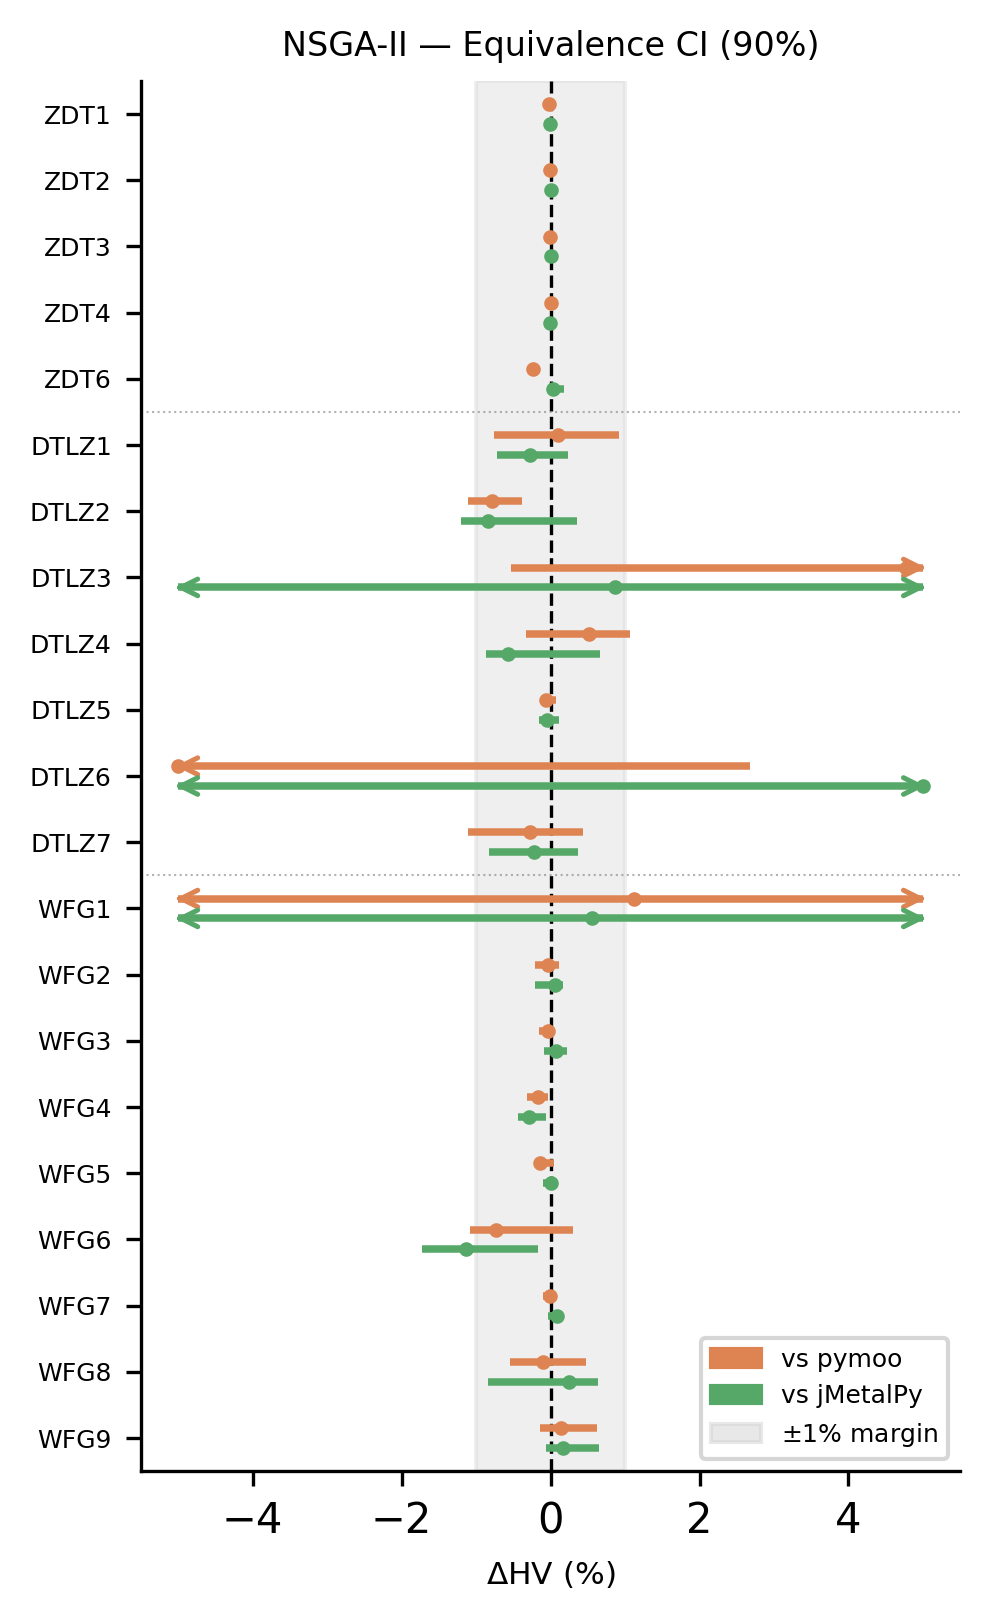
\includegraphics[width=\columnwidth]{figures/forest_ci_nsgaii.png}
  \caption{NSGA-II. Per-problem paired bootstrap 90\% confidence intervals for the relative normalized hypervolume difference $\Delta = (\HV_{\text{\VAMOS}} - \HV_{\text{fw}})/\HV_{\text{fw}}$, reported in percent. The shaded band marks the $\pm 1\%$ equivalence margin; intervals falling entirely within this band indicate statistical equivalence}
  \label{fig:forest_ci_nsgaii}
\end{figure}




\begin{table}[htbp]
\centering
\caption{NSGA-II. Normalized hypervolume comparison with Wilcoxon signed-rank test results (Holm-corrected)}
\label{tab:stats_hypervolume_nsgaii}
\begin{tabular}{lccccc}
\toprule
\textbf{Problem} & \textbf{VAMOS} & \textbf{pymoo} & \textbf{p-value} & \textbf{$\hat{A}_{12}$} & \textbf{Significance} \\
\midrule
dtlz1 & 0.920 & \textbf{0.921} & 1.000 & 0.47 & \xmark \\
dtlz2 & 0.826 & \textbf{0.827} & 1.000 & 0.46 & \xmark \\
dtlz3 & \textbf{0.749} & 0.673 & 0.813 & 0.66 & \xmark \\
dtlz4 & 0.828 & \textbf{0.829} & 1.000 & 0.49 & \xmark \\
dtlz5 & 0.966 & \textbf{0.966} & 1.000 & 0.45 & \xmark \\
dtlz6 & 0.444 & \textbf{0.510} & 1.000 & 0.32 & \xmark \\
dtlz7 & \textbf{0.876} & 0.874 & 1.000 & 0.53 & \xmark \\
wfg1 & 0.353 & \textbf{0.430} & 1.000 & 0.36 & \xmark \\
wfg2 & 1.007 & \textbf{1.007} & 1.000 & 0.37 & \xmark \\
wfg3 & 0.971 & \textbf{0.973} & 1.000 & 0.35 & \xmark \\
wfg4 & 0.956 & \textbf{0.957} & 1.000 & 0.48 & \xmark \\
wfg5 & 0.826 & \textbf{0.826} & 0.513 & 0.32 & \xmark \\
wfg6 & 0.840 & \textbf{0.846} & 1.000 & 0.44 & \xmark \\
wfg7 & 0.963 & \textbf{0.964} & 1.000 & 0.41 & \xmark \\
wfg8 & \textbf{0.745} & 0.745 & 1.000 & 0.54 & \xmark \\
wfg9 & 0.714 & \textbf{0.714} & 1.000 & 0.48 & \xmark \\
zcat1 & 0.983 & \textbf{0.983} & 1.000 & 0.44 & \xmark \\
zcat10 & 0.951 & \textbf{0.951} & 1.000 & 0.43 & \xmark \\
zcat11 & 0.990 & \textbf{0.990} & 1.000 & 0.48 & \xmark \\
zcat12 & 0.989 & \textbf{0.990} & 1.000 & 0.45 & \xmark \\
zcat13 & 1.016 & \textbf{1.016} & 1.000 & 0.47 & \xmark \\
zcat14 & 0.977 & \textbf{0.977} & 1.000 & 0.36 & \xmark \\
zcat15 & 0.989 & \textbf{0.990} & 1.000 & 0.45 & \xmark \\
zcat16 & 0.987 & \textbf{0.988} & 1.000 & 0.40 & \xmark \\
zcat17 & 0.995 & \textbf{0.995} & 1.000 & 0.46 & \xmark \\
zcat18 & \textbf{0.990} & 0.990 & 1.000 & 0.52 & \xmark \\
zcat19 & 0.986 & \textbf{0.986} & 1.000 & 0.42 & \xmark \\
zcat2 & 0.992 & \textbf{0.992} & 1.000 & 0.49 & \xmark \\
zcat20 & \textbf{0.990} & 0.990 & 1.000 & 0.52 & \xmark \\
zcat3 & 0.983 & \textbf{0.983} & 1.000 & 0.37 & \xmark \\
zcat4 & 0.983 & \textbf{0.983} & 1.000 & 0.37 & \xmark \\
zcat5 & 0.995 & \textbf{0.995} & 1.000 & 0.46 & \xmark \\
zcat6 & 0.995 & \textbf{0.995} & 1.000 & 0.46 & \xmark \\
zcat7 & \textbf{0.990} & 0.990 & 1.000 & 0.52 & \xmark \\
zcat8 & 0.971 & \textbf{0.971} & 1.000 & 0.49 & \xmark \\
zcat9 & 0.971 & \textbf{0.971} & 1.000 & 0.49 & \xmark \\
zdt1 & 0.991 & \textbf{0.991} & 1.000 & 0.42 & \xmark \\
zdt2 & 0.982 & \textbf{0.982} & 1.000 & 0.44 & \xmark \\
zdt3 & 0.996 & \textbf{0.996} & 1.000 & 0.55 & \xmark \\
zdt4 & 1.001 & \textbf{1.001} & 1.000 & 0.43 & \xmark \\
zdt6 & 0.982 & \textbf{0.986} & $<$0.0001 & 0.00 & \cmark \\
\bottomrule
\end{tabular}
\end{table}

\begin{table}[htbp]
\centering
\caption{NSGA-II. IGD+ comparison with Wilcoxon signed-rank test results (Holm-corrected). Lower is better}
\label{tab:stats_igd_plus_nsgaii}
\begin{tabular}{lccccc}
\toprule
\textbf{Problem} & \textbf{VAMOS} & \textbf{pymoo} & \textbf{p-value} & \textbf{$\hat{A}_{12}$} & \textbf{Significance} \\
\midrule
dtlz1 & 0.0181 & \textbf{0.0179} & 1.000 & 0.53 &  \xmark \\
dtlz2 & 0.0357 & \textbf{0.0352} & 1.000 & 0.56 &  \xmark \\
dtlz3 & \textbf{0.0518} & 0.0716 & 0.834 & 0.32 &  \xmark \\
dtlz4 & 0.0357 & \textbf{0.0351} & 1.000 & 0.54 &  \xmark \\
dtlz5 & 0.0029 & \textbf{0.0029} & 1.000 & 0.51 &  \xmark \\
dtlz6 & 0.0996 & \textbf{0.0837} & 1.000 & 0.67 &  \xmark \\
dtlz7 & 0.0350 & \textbf{0.0350} & 1.000 & 0.56 &  \xmark \\
wfg1 & 0.7451 & \textbf{0.6949} & 1.000 & 0.65 &  \xmark \\
wfg2 & 0.2162 & \textbf{0.2155} & 1.000 & 0.64 &  \xmark \\
wfg3 & 0.0206 & \textbf{0.0191} & 1.000 & 0.65 &  \xmark \\
wfg4 & 0.0133 & \textbf{0.0128} & 1.000 & 0.53 &  \xmark \\
wfg5 & \textbf{0.0699} & 0.0700 & 1.000 & 0.51 &  \xmark \\
wfg6 & 0.0600 & \textbf{0.0573} & 1.000 & 0.59 &  \xmark \\
wfg7 & 0.0106 & \textbf{0.0103} & 1.000 & 0.58 &  \xmark \\
wfg8 & \textbf{0.1463} & 0.1485 & 1.000 & 0.45 &  \xmark \\
wfg9 & \textbf{0.1263} & 0.1264 & 1.000 & 0.51 &  \xmark \\
zcat1 & 0.0074 & \textbf{0.0073} & 1.000 & 0.58 &  \xmark \\
zcat10 & 0.0033 & \textbf{0.0032} & 1.000 & 0.57 &  \xmark \\
zcat11 & 0.0049 & \textbf{0.0049} & 1.000 & 0.49 &  \xmark \\
zcat12 & 0.0050 & \textbf{0.0049} & 1.000 & 0.52 &  \xmark \\
zcat13 & 0.0038 & \textbf{0.0037} & 1.000 & 0.57 &  \xmark \\
zcat14 & 0.0070 & \textbf{0.0069} & 1.000 & 0.64 &  \xmark \\
zcat15 & 0.0050 & \textbf{0.0050} & 1.000 & 0.52 &  \xmark \\
zcat16 & 0.0048 & \textbf{0.0046} & 1.000 & 0.58 &  \xmark \\
zcat17 & 0.0040 & \textbf{0.0040} & 1.000 & 0.51 &  \xmark \\
zcat18 & \textbf{0.0044} & 0.0044 & 1.000 & 0.51 &  \xmark \\
zcat19 & 0.0062 & \textbf{0.0061} & 1.000 & 0.58 &  \xmark \\
zcat2 & 0.0059 & \textbf{0.0059} & 1.000 & 0.52 &  \xmark \\
zcat20 & \textbf{0.0045} & 0.0045 & 1.000 & 0.52 &  \xmark \\
zcat3 & 0.0074 & \textbf{0.0072} & 1.000 & 0.63 &  \xmark \\
zcat4 & 0.0074 & \textbf{0.0072} & 1.000 & 0.63 &  \xmark \\
zcat5 & 0.0040 & \textbf{0.0040} & 1.000 & 0.53 &  \xmark \\
zcat6 & 0.0027 & \textbf{0.0026} & 1.000 & 0.63 &  \xmark \\
zcat7 & \textbf{0.0044} & 0.0044 & 1.000 & 0.52 &  \xmark \\
zcat8 & 0.0057 & \textbf{0.0056} & 1.000 & 0.51 &  \xmark \\
zcat9 & 0.0057 & \textbf{0.0057} & 1.000 & 0.50 &  \xmark \\
zdt1 & 0.0032 & \textbf{0.0031} & 1.000 & 0.53 &  \xmark \\
zdt2 & 0.0030 & \textbf{0.0030} & 1.000 & 0.53 &  \xmark \\
zdt3 & \textbf{0.0015} & 0.0015 & 1.000 & 0.45 &  \xmark \\
zdt4 & 0.0008 & \textbf{0.0008} & 1.000 & 0.59 &  \xmark \\
zdt6 & 0.0031 & \textbf{0.0024} & $<$0.0001 & 1.00 & \checkmark \\
\bottomrule
\end{tabular}
\end{table}

\begin{table}[htbp]
\centering
\caption{Normalized hypervolume equivalence summary (paired bootstrap 90\% CI; equivalence margin $\pm 1\%$ relative)}
\label{tab:hv_equivalence_summary_nsgaii}
\resizebox{\columnwidth}{!}{%
\begin{tabular}{lccc}
\toprule
\textbf{Framework} & \textbf{Eq.\ problems} & \textbf{Non-inf.\ problems} & \textbf{Median $\Delta$HV (\%)} \\
\midrule
\textit{pymoo} & 37/41 & 38/41 & -0.01 \\
\textit{jMetalPy} & 35/41 & 35/41 & -0.02 \\
\textit{DEAP} & 33/41 & 37/41 & -0.01 \\
\textit{Platypus} & 33/41 & 38/41 & +0.05 \\
\bottomrule
\end{tabular}%
}
\end{table}

\begin{table}[htbp]
\centering
\caption{Robustness summary for normalized hypervolume across seeds (median across problems). ``Near-best'' is defined per problem as HV $\ge 0.99 \cdot \max$ median(HV) among frameworks}
\label{tab:hv_robustness_summary_nsgaii}
\begin{tabular}{lcc}
\toprule
\textbf{Framework} & \textbf{Median IQR(HV)} & \textbf{Median \% seeds near-best} \\
\midrule
VAMOS & 0.001 & 100.0 \\
\textit{pymoo} & 0.001 & 100.0 \\
\textit{jMetalPy} & 0.002 & 100.0 \\
\textit{DEAP} & 0.001 & 100.0 \\
\textit{Platypus} & 0.001 & 100.0 \\
\bottomrule
\end{tabular}
\end{table}

\begin{figure}[htbp]
  \centering
  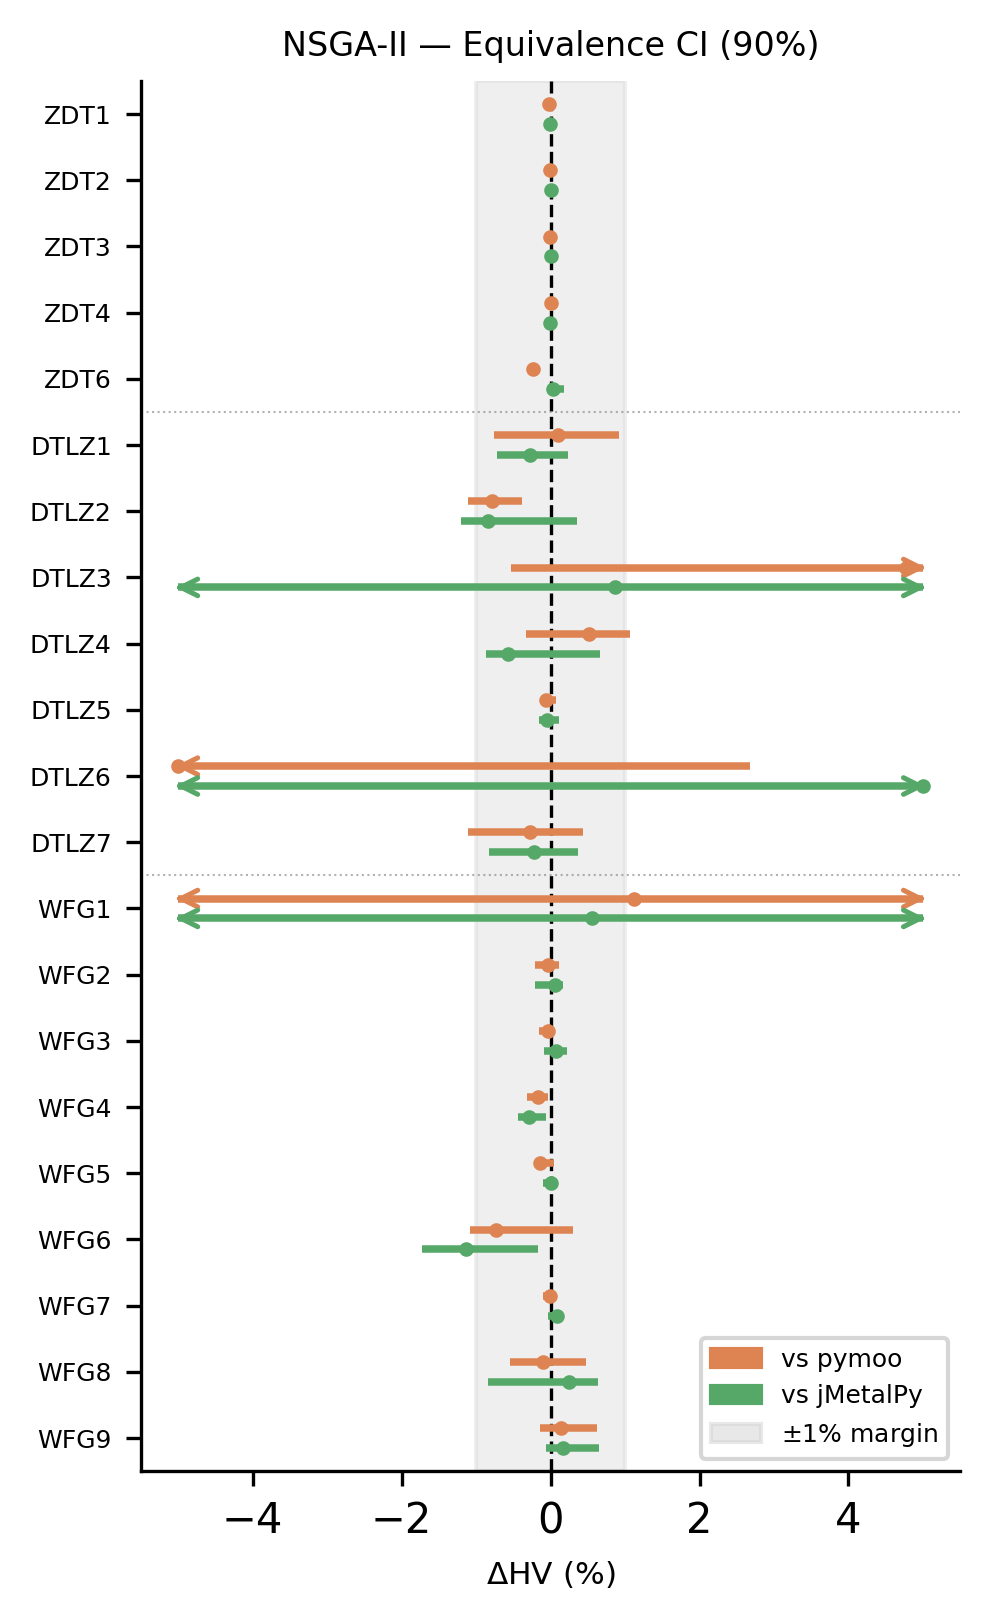
\includegraphics[width=\columnwidth]{figures/forest_ci_nsgaii.png}
  \caption{NSGA-II. Per-problem paired bootstrap 90\% confidence intervals for the relative normalized hypervolume difference $\Delta = (\HV_{\text{\VAMOS}} - \HV_{\text{fw}})/\HV_{\text{fw}}$, reported in percent. The shaded band marks the $\pm 1\%$ equivalence margin; intervals falling entirely within this band indicate statistical equivalence}
  \label{fig:forest_ci_nsgaii}
\end{figure}
